\subsection{Preprocessing}

\begin{frame}{Preprocessing}
    \tikzstyle{block} = [rectangle, draw, fill=orange!40, 
    text width=5em, text centered, minimum height=4em]
    \tikzstyle{line} = [draw, -\darkarrow]
    \newcommand*\activelinewidth{0.5mm}
    \begin{center}
    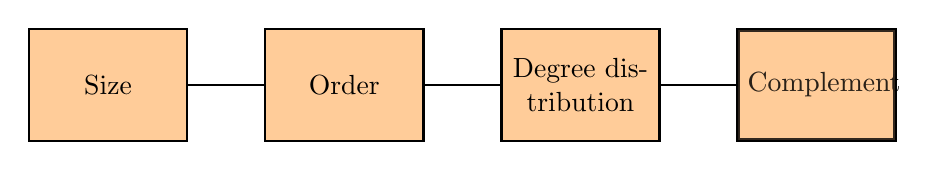
\begin{tikzpicture}[node distance = 3cm]
        \node<1>[block, line width = \activelinewidth] (start) {Size};
        \node<2->[block, line width = 0.15mm] (start) {Size};
        \node<2>[block, line width = \activelinewidth ,right of=start](order) {Order};
        \node<1>[block, line width = 0.15mm ,right of=start, opacity = 0.2](order) {Order};
        \node<3->[block, line width = 0.15mm ,right of=start](order) {Order};
        \node<3>[block, line width = \activelinewidth,right of=order](degree) {Degree distribution};
        \node<1-2>[block, line width = 0.15mm,right of=order, opacity = 0.2](degree) {Degree distribution};
        \node<4->[block, line width = 0.15mm,right of=order](degree) {Degree distribution};
        \node<4>[block, line width = \activelinewidth,right of=degree] (compl) {Complement};
        \node<1-3>[block, line width = 0.15mm,right of=degree, opacity = 0.2] (compl) {Complement};
        % % Draw edges
        \path<1>[line,opacity = 0.2] (start) -- (order);
        \path<1-2>[line,opacity = 0.2] (order) -- (degree);
        \path<1-3>[line,opacity = 0.2] (degree) -- (compl);
        \path<2->[line] (start) -- (order);
        \path<3->[line] (order) -- (degree);
        \path<4->[line] (degree) -- (compl);
    \end{tikzpicture}
    \end{center}
    \only<1-3>{
        \begin{figure}
        \begin{tikzpicture}
            \Vertices{circle}{A,B,C}
            \Edges(A,B,C)
        \end{tikzpicture}
        \caption{\only<1>{Size = 2}
        \only<2>{Order = 3}
        \only<3>{deg = 1: (A,C), deg = 2: (B)}}
        \end{figure}
    }
    \only<4>{
    \begin{figure}
    \begin{minipage}{0.35\textwidth}
        \centering
        \begin{tikzpicture}
            \Vertices{square}{A,B,C,D}
            \Edges(A,C,B,D,A)
        \end{tikzpicture}
        \caption{Original graph}
    \end{minipage}
    \begin{minipage}{0.35\textwidth}
        \centering
        \begin{tikzpicture}
            \Vertices{square}{A,B,C,D}
            \Edge(C)(D)
            \Edge(A)(B)
        \end{tikzpicture}
    \caption{Complement}
    \end{minipage}
    \end{figure}
    }
\end{frame}
